
\documentclass[a4paper,12pt]{article}

%%% Работа с русским языком
\usepackage{cmap}					% поиск в PDF
\usepackage{mathtext} 				% русские буквы в формулах
\usepackage[T2A]{fontenc}			% кодировка
\usepackage[utf8]{inputenc}			% кодировка исходного текста
\usepackage[english, russian]{babel}	% локализация и переносы
\usepackage{indentfirst}
\frenchspacing
\usepackage{amsmath} 
\usepackage{amsfonts}
\usepackage{amssymb}

\newcommand{\bz}{\mathbf{z}}
\newcommand{\bx}{\mathbf{x}}
\newcommand{\by}{\mathbf{y}}
\newcommand{\bv}{\mathbf{v}}
\newcommand{\bw}{\mathbf{w}}
\newcommand{\ba}{\mathbf{a}}
\newcommand{\bb}{\mathbf{b}}
\newcommand{\bp}{\mathbf{p}}
\newcommand{\bq}{\mathbf{q}}
\newcommand{\bt}{\mathbf{t}}
\newcommand{\bu}{\mathbf{u}}
\newcommand{\bT}{\mathbf{T}}
\newcommand{\bX}{\mathbf{X}}
\newcommand{\bZ}{\mathbf{Z}}
\newcommand{\bS}{\mathbf{S}}
\newcommand{\bH}{\mathbf{H}}
\newcommand{\bW}{\mathbf{W}}
\newcommand{\bY}{\mathbf{Y}}
\newcommand{\bU}{\mathbf{U}}
\newcommand{\bQ}{\mathbf{Q}}
\newcommand{\bP}{\mathbf{P}}
\newcommand{\bA}{\mathbf{A}}
\newcommand{\bB}{\mathbf{B}}
\newcommand{\bC}{\mathbf{C}}
\newcommand{\bE}{\mathbf{E}}
\newcommand{\bF}{\mathbf{F}}
\newcommand{\bomega}{\boldsymbol{\omega}}
\newcommand{\btheta}{\boldsymbol{\theta}}
\newcommand{\bgamma}{\boldsymbol{\gamma}}
\newcommand{\bdelta}{\boldsymbol{\delta}}
%\newcommand{\bPsi}{\boldsymbol{\Psi}}
%\newcommand{\bpsi}{\boldsymbol{\psi}}
\newcommand{\bxi}{\boldsymbol{\xi}}
\newcommand{\bchi}{\boldsymbol{\chi}}
\newcommand{\bzeta}{\boldsymbol{\zeta}}
\newcommand{\blambda}{\boldsymbol{\lambda}}
\newcommand{\beps}{\boldsymbol{\varepsilon}}
\newcommand{\bZeta}{\boldsymbol{Z}}
% mathcal
\newcommand{\cX}{\mathcal{X}}
\newcommand{\cY}{\mathcal{Y}}
\newcommand{\cW}{\mathcal{W}}

\newcommand{\dH}{\mathbb{H}}
\newcommand{\dR}{\mathbb{R}}
% transpose
\newcommand{\T}{^{\mathsf{T}}}

\renewcommand{\epsilon}{\ensuremath{\varepsilon}}
%\renewcommand{\phi}{\ensuremath{\varphi}}
\renewcommand{\kappa}{\ensuremath{\varkappa}}
\renewcommand{\le}{\ensuremath{\leqslant}}
\renewcommand{\leq}{\ensuremath{\leqslant}}
\renewcommand{\ge}{\ensuremath{\geqslant}}
\renewcommand{\geq}{\ensuremath{\geqslant}}
\renewcommand{\emptyset}{\varnothing}

%%% Дополнительная работа с математикой
\usepackage{amsmath,amsfonts,amssymb,amsthm,mathtools} % AMS
\usepackage{icomma} % "Умная" запятая: $0,2$ --- число, $0, 2$ --- перечисление

%% Номера формул
%\mathtoolsset{showonlyrefs=true} % Показывать номера только у тех формул, на которые есть \eqref{} в тексте.
%\usepackage{leqno} % Нумереация формул слева

%% Свои команды
\DeclareMathOperator{\sgn}{\mathop{sgn}}

%% Перенос знаков в формулах (по Львовскому)
\newcommand*{\hm}[1]{#1\nobreak\discretionary{}
	{\hbox{$\mathsurround=0pt #1$}}{}}

%%% Работа с картинками
\usepackage{graphicx}  % Для вставки рисунков
\setlength\fboxsep{3pt} % Отступ рамки \fbox{} от рисунка
\setlength\fboxrule{1pt} % Толщина линий рамки \fbox{}
\usepackage{wrapfig} % Обтекание рисунков текстом

%%% Работа с таблицами
\usepackage{array,tabularx,tabulary,booktabs} % Дополнительная работа с таблицами
\usepackage{longtable}  % Длинные таблицы
\usepackage{multirow} % Слияние строк в таблице

%%% Теоремы
\theoremstyle{plain} % Это стиль по умолчанию, его можно не переопределять.
\newtheorem{theorem}{Теорема}[section]
\newtheorem{proposition}[theorem]{Утверждение}

\theoremstyle{definition} % "Определение"
\newtheorem{corollary}{Следствие}[theorem]
\newtheorem{problem}{Задача}[section]

\theoremstyle{remark} % "Примечание"
\newtheorem*{nonum}{Решение}

%%% Программирование
\usepackage{etoolbox} % логические операторы

%%% Страница
\usepackage{extsizes} % Возможность сделать 14-й шрифт
\usepackage{geometry} % Простой способ задавать поля
\geometry{top=25mm}
\geometry{bottom=35mm}
\geometry{left=35mm}
\geometry{right=20mm}
%
%\usepackage{fancyhdr} % Колонтитулы
% 	\pagestyle{fancy}
%\renewcommand{\headrulewidth}{0pt}  % Толщина линейки, отчеркивающей верхний колонтитул
% 	\lfoot{Нижний левый}
% 	\rfoot{Нижний правый}
% 	\rhead{Верхний правый}
% 	\chead{Верхний в центре}
% 	\lhead{Верхний левый}
%	\cfoot{Нижний в центре} % По умолчанию здесь номер страницы

\usepackage{setspace} % Интерлиньяж
%\onehalfspacing % Интерлиньяж 1.5
%\doublespacing % Интерлиньяж 2
%\singlespacing % Интерлиньяж 1

\usepackage{lastpage} % Узнать, сколько всего страниц в документе.

\usepackage{soul} % Модификаторы начертания

\usepackage{hyperref}
\usepackage[usenames,dvipsnames,svgnames,table,rgb]{xcolor}
\hypersetup{				% Гиперссылки
	unicode=true,           % русские буквы в раздела PDF
	pdftitle={Заголовок},   % Заголовок
	pdfauthor={Автор},      % Автор
	pdfsubject={Тема},      % Тема
	pdfcreator={Создатель}, % Создатель
	pdfproducer={Производитель}, % Производитель
	pdfkeywords={keyword1} {key2} {key3}, % Ключевые слова
	colorlinks=true,       	% false: ссылки в рамках; true: цветные ссылки
	linkcolor=red,          % внутренние ссылки
	citecolor=black,        % на библиографию
	filecolor=magenta,      % на файлы
	urlcolor=cyan           % на URL
}

\usepackage{csquotes} % Еще инструменты для ссылок

%\usepackage[style=authoryear,maxcitenames=2,backend=biber,sorting=nty]{biblatex}

\usepackage{multicol} % Несколько колонок

\usepackage{tikz} % Работа с графикой
\usepackage{pgfplots}
\usepackage{pgfplotstable}


\begin{document}

\title{Machine learning models for Navier-Stocks}
\author{Боева Галина, группа М05-304а}
\date{\today}

\maketitle
\section{Введение}
Симуляция физических процессов, таких как движение жидкостей, является важной задачей в науке и инженерии. Традиционные методы часто используют графовые структуры для определения взаимодействий между частицами, что может быть неэффективно для описания непрерывных процессов, таких как механика жидкостей. В данной статье авторы предлагают альтернативный подход, основанный на лагранжевой модели и непрерывных свертках, что позволяет более точно и быстро моделировать поведение жидкостей.
\section{Основные подходы в теме}
Лагранжева модель: Использует набор частиц для представления жидкости, где каждая частица несет локальные свойства, такие как скорость и плотность.

Методы сглаженной гидродинамики (SPH): Популярный подход для моделирования жидкостей, который использует частичные дифференциальные уравнения для описания динамики.

Графовые структуры: Традиционные методы используют графы для определения взаимодействий между частицами, что может усложнять модель при больших масштабах.
\subsection{Лагранжевые координаты}
Лагранжевые координаты описывают положение частиц или элементов системы в зависимости от времени. Если $\mathbf{x}_i(t)$ — положение частицы $i$ в момент времени $t$, то её скорость $\mathbf{v}_i(t)$ определяется как производная по времени:

\begin{equation}
\mathbf{v}_i(t) = \frac{d\mathbf{x}_i(t)}{dt}
\end{equation}

\subsection{Уравнения движения}
Уравнения движения для частиц в лагранжевых координатах могут быть записаны в виде:

\begin{equation}
\frac{d\mathbf{x}_i(t)}{dt} = \mathbf{v}_i(t)
\end{equation}

\begin{equation}
\frac{d\mathbf{v}_i(t)}{dt} = \mathbf{a}_i(t)
\end{equation}

где $\mathbf{a}_i(t)$ — ускорение частицы $i$, которое может зависеть от различных сил, действующих на частицу.

\section{Основные формулы и алгоритм действий}
\subsection{Непрерывные свертки}

Авторы рассматривают жидкости как пространственно непрерывные функции, отобранные в конечном наборе (непрерывно меняющихся) положений, и обрабатывают их с помощью нового слоя непрерывной свертки. Это более точно соответствует непрерывному характеру задачи и упрощает определение нейронных сетей за счет абстрагирования от представления частиц, лежащего в их основе.

Авторы расширили представление фильтров на основе сетки, обычно используемое для дискретных сверток, до непрерывной области с помощью простой линейной интерполяции. Линейная интерполяция фильтров позволяет эффективно искать пространственно изменяющиеся значения фильтров в произвольных точках, сохраняя при этом компактность и эффективность представления в виде сетки. Кроме того, авторы используют функцию окна для определения поддержки фильтров и отображение шара в куб для поддержки сферических полей восприятия.

Авторы показали, что их свертки, несмотря на их простоту, работают лучше, чем более сложные представления.
\subsection{Уравнения Навье-Стокса}
Жидкости изучаются уже несколько веков, и уравнения Навье-Стокса для несжимаемых жидкостей хорошо установлены (Батчелор, 1967):

\begin{equation}
\frac{\partial \mathbf{v}}{\partial t} + \mathbf{v} \cdot \nabla \mathbf{v} = -\frac{1}{\rho} \nabla p + \nu \nabla^2 \mathbf{v} + \mathbf{g}, \quad \text{при условии} \quad \nabla \cdot \mathbf{v} = 0.
\end{equation}

\section{Метод решения}
Одним из распространенных методов решения этих дифференциальных уравнений является аппроксимация жидкости набором гладких частиц. Каждая частица соответствует непрерывному объему вещества и несет локальные свойства жидкости, такие как скорость и плотность, которые движутся с потоком. Это мотивировано тем, что функция $A(\mathbf{x})$ может быть представлена интегральной интерполяцией:

\begin{equation}
A(\mathbf{x}) = \int A(\mathbf{x}') \delta(\|\mathbf{x} - \mathbf{x}'\|^2) dV(\mathbf{x}'),
\end{equation}

где $\delta(\mathbf{x})$ обозначает дельта-функцию Дирака. Это уравнение может быть дискретизировано как:

\begin{equation}
A(\mathbf{x}) \approx \sum_i V_i A_i W(\|\mathbf{x} - \mathbf{x}'\|^2, h),
\end{equation}

где $V_i$ — объем в данной точке пространства, и

\begin{equation}
\lim_{h \to 0} W(\|\mathbf{x} - \mathbf{x}'\|, h) = \delta(\|\mathbf{x} - \mathbf{x}'\|).
\end{equation}

Здесь $W(\mathbf{x}, h)$ — гладкое ядро или свертка с радиусом $h$, обычно в виде гауссового распределения, но могут использоваться и более сложные функции. В практике ядро конечно и дает локализованные окрестности частиц, которые взаимодействуют через взаимодействия, взвешенные производными ядра. Таким образом, непрерывное описание жидкостей из уравнения (1) может быть дискретизировано в лагранжевом виде и решено численно. Обычно внутренние силы рассчитываются на основе локального давления, вязкости и поверхностного натяжения, что дает обновление для положения каждой частицы.
\section{Дискретная свертка}
Оператор дискретной свертки, обычно используемый в ConvNets, определяется как:

\begin{equation}
(f * g)(x) = \sum_{\tau \in \Omega} f(x + \tau) g(\tau),
\end{equation}

где $f$ и $g$ — входная функция и фильтр, $x$ — положение, $\tau$ — вектор сдвига, а $\Omega$ — множество векторов сдвига, определяющее поддержку фильтра. На регулярных данных, таких как изображения, положения $x$ варьируются по регулярной сетке, а векторы сдвига $\tau$ являются целочисленными, т.е. $x, \tau \in \mathbb{Z}^d$ для некоторой размерности $d$. Аналогично в непрерывной области эта свертка определяется как:

\begin{equation}
(f * g)(x) = \int_{\mathbb{R}^d} f(x + \tau) g(\tau) d\tau,
\end{equation}

где $x$ и $\tau$ — вещественные векторы, т.е. $x, \tau \in \mathbb{R}^d$.

\section{Адаптация к неструктурированным облакам точек}
Теперь адаптируем это определение к неструктурированным облакам точек. В этом случае у нас есть конечное число точек, которые дискретизируют функцию $f$, но не лежат на сетке. Для облака точек с $i = 1, \ldots, N$ точками со значениями $f_i$ в положениях $x_i$, мы определяем свертку в положении $x$ как:

\begin{equation}
(f * g)(x) = \frac{1}{\psi(x)} \sum_{i \in N(x, R)} a(x_i, x) f_i g(\Lambda(x_i - x)),
\end{equation}

где $N(x, R)$ — множество точек в радиусе $R$ вокруг $x$. $a$ — скалярная функция, которая может использоваться для нормализации плотности, специфичной для точек $x_i$ и $x$. В простейшем случае $a$ может быть постоянной: $a = 1$. В нашем случае мы хотим обеспечить плавный отклик нашей свертки при изменении соседства частиц, поэтому определяем $a$ как функцию окна:

\begin{equation}
a(x_i, x) = \left(1 - \frac{\|x_i - x\|^2}{2R^2}\right)^3 \quad \text{если} \quad \|x_i - x\|^2 < R,
\end{equation}

иначе $a(x_i, x) = 0$. $\psi$ — еще одна скалярная функция для нормализации, которая может быть установлена в нашей реализации как:

\begin{equation}
\psi(x) = 1 \quad \text{или} \quad \psi(x) = \sum_{i \in N(x, R)} a(x_i, x).
\end{equation}
\begin{figure}
    \centering
    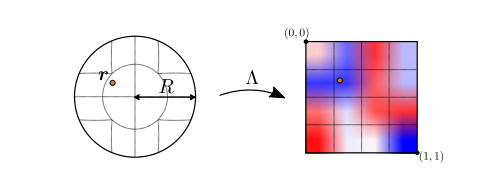
\includegraphics[width=0.5\linewidth]{essay4_1.png}
    \caption{Используются сферические формы фильтров для наших непрерывных сверток, но используем обычные сетки для хранения значений фильтров. В левой части рисунка показана сферическая область радиусом $R$ и точка
с относительными координатами \textbf{r} относительно центра. Далее слудет преобразование \textbf{r} через отображение $\Lambda$  в нормализованные
координаты в обычной сетке. Тонкие пунктирные линии иллюстрируют искажение отображения. Для поиска
конечного значения фильтра мы используем трехлинейную интерполяцию в обычной сетке.}
    \label{fig:enter-label}
\end{figure}
Авторы используют $\psi(x) = 1$, так как изменения в плотности частиц являются важной особенностью для моделирования жидкостей. Для фильтра $g$ они просто используют регулярную сетку для хранения значений фильтра, но применяют линейную интерполяцию, чтобы сделать $g$ непрерывной функцией. Кроме того, авторы используют отображение $\Lambda(r)$ единичного шара в единичный куб для реализации сферических фильтров, как показано на рисунке 1. Промежуточное отображение координат $\Lambda$ предоставляет гибкость для реализации различных пространственных форм, сохраняя при этом преимущества регулярной сетки для хранения и поиска значений фильтра.

\section{Обучение механики жидкостей}
Наша цель — изучить механику жидкостей, наблюдая за движением частиц. Входными данными для нашей ConvNet является набор частиц с соответствующими характеристиками. Поскольку положение само по себе не является характеристикой, а просто определяет положение частицы в пространстве, мы должны присвоить каждой частице вектор характеристик. Вектор характеристик, который мы используем, состоит из постоянного скаляра 1, скорости $v$ и вязкости $\nu$. Таким образом, частица $p_i$ на шаге $n$ с её положением и вектором характеристик представляет собой кортеж $(x_n^i, [1, v_n^i, \nu_i])$.

Определение скорости в явном виде как входной характеристики позволяет нам вычислять промежуточные скорости и положения, и применять внешние силы, передавая эту информацию в сеть. Мы вычисляем промежуточные положения $x_n^{*i}$ и скорости $v_n^{*i}$, начиная с шага $n$, с помощью метода Хьюна:

\begin{equation}
v_n^{*i} = v_n^i + \Delta t a_{\text{ext}}
\end{equation}

\begin{equation}
x_n^{*i} = x_n^i + \Delta t \left(v_n^i + \frac{v_n^{*i}}{2}\right).
\end{equation}

Вектор $a_{\text{ext}}$ — ускорение, через которое мы можем применять внешние силы для управления жидкостью или просто применять гравитацию. Промежуточные положения и скорости не учитывают взаимодействия между частицами или сценой, которые будем реализовывать с помощью ConvNet. Чтобы позволить сети обрабатывать столкновения с окружением, мы определяем второй набор статических частиц $s_j$. Мы выбираем частицы на границах сцены с нормалями $n_j$ как векторы характеристик, т.е. $s_j = (x_j, [n_j])$.

Сеть реализует функцию:

\begin{equation}
[\Delta x_1, \ldots, \Delta x_N] = \text{ConvNet}(\{p_n^{*1}, \ldots, p_n^{*N}\}, \{s_1, \ldots, s_M\}),
\end{equation}

которая использует свертки для комбинирования характеристик из обоих наборов частиц. $\Delta x$ — коррекция положения, которая учитывает все взаимодействия частиц, включая обработку столкновений со сценой. Наконец, применяется коррекцию для обновления положений и скоростей для шага $n + 1$:

\begin{equation}
x_{n+1}^i = x_n^{*i} + \Delta x_i
\end{equation}

\begin{equation}
v_{n+1}^i = \frac{x_{n+1}^i - x_n^i}{\Delta t}.
\end{equation}

Обратите внимание, что обновленное положение $x_{n+1}^i$ зависит от вектора выхода $\Delta x_i$ и позволяет непосредственно определять нашу цель обучения на основе положений частиц.
\begin{figure}
    \centering
    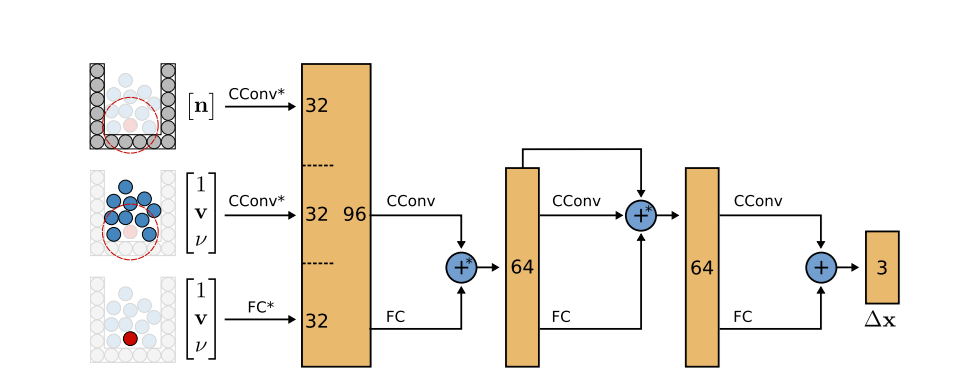
\includegraphics[width=0.8\linewidth]{essay4_2.png}
    \caption{Схема сети.}
    \label{fig:enter-label}
\end{figure}

\begin{figure}
    \centering
    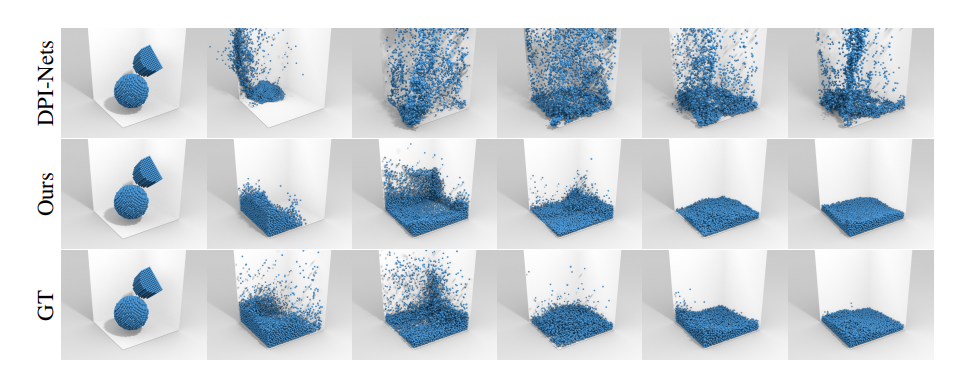
\includegraphics[width=0.8\linewidth]{essay4_3.png}
    \caption{Пример работы.}
    \label{fig:enter-label}
\end{figure}

\section{Заключение}
Предложенный подход~\cite{ummenhofer2019lagrangian} позволяет эффективно моделировать жидкости с использованием непрерывных сверток в нейронных сетях. Это улучшает точность и скорость симуляции по сравнению с традиционными графовыми методами. Еще интересная практическая работа представлена в~\cite{sanchez2020learning}.



\bibliographystyle{unsrt}
\bibliography{references-final}
\end{document}
